\clearpage
\section{Image reconstruction in the frequency domain}

In the following section, reconstructing an image based on the inverse of the degradation will be examined.

\subsection{Restoring an image using the inverse of a degradation}

\subsubsection{Compare the restored image with the original image and the blurred image. How does the restored image and the PSNR differ from the blurred image? Is it better or worse? Why?}

The blurred image is simply a blurred version of the original image, created using a averaging filter. The restored image appears identical to the original image. The PSNR of +251.54dB corresponds to a MSE in the image of $\leq 3\times{10}^{-11}$; which is likely due to the limited precision of MATLAB. As the blur operation is a linear-position-invariant filter, it is easily reversible and the image we restore is basically identical to the original.


\begin{figure}[ht]
\centering
	\subfigure[Base image]{
	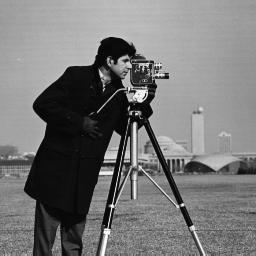
\includegraphics[width=0.30\textwidth]{question6/1_camBase}
	}
	\subfigure[Blurred image; PSNR +16.90]{
	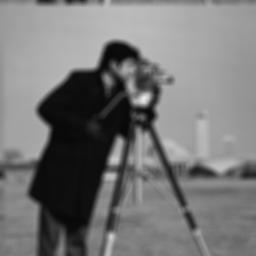
\includegraphics[width=0.30\textwidth]{question6/1_cam_blur}
	}
	\subfigure[Image reconstructed using blur inverse; PSNR +251.54dB]{
	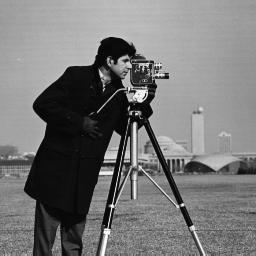
\includegraphics[width=0.30\textwidth]{question6/1_cam_unblur}
	}
	\caption{The base cameraman image has been degraded using a disk blur filter with a radius of 4.}
\end{figure}

\clearpage
\subsection{Noise and image restoration using the inverse}
Gaussian noise has been added to the image after it has been blurred. Applying the inverse blur operation may not be able to restore the image to it's original state.

\begin{figure}[ht]
\centering
	\subfigure[Blurred image; PSNR +16.90]{
	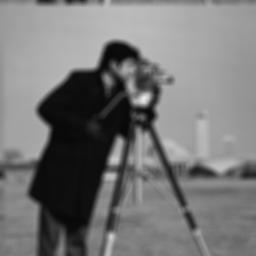
\includegraphics[width=0.30\textwidth]{question6/1_cam_blur}
	}
	\subfigure[Gaussian noise, $\sigma^2$=0.002; PSNR +16.50]{
	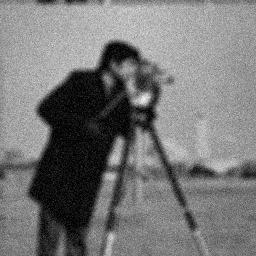
\includegraphics[width=0.30\textwidth]{question6/2_cam_blur_noisy}
	}
	\subfigure[Image reconstructed using blur inverse; PSNR -35.24dB]{
	
\includegraphics[width=0.30\textwidth]{question6/2_cam_unblur_noisy}
	}
\end{figure}


\subsubsection{Compare the restored image with the restored image from the previous step. How does the restored image and the PSNR differ from the previous restored image? Is it better or worse? Why?}

This restored image looks nothing like the original image. While the blurred images with and without noise appear very similar and have very similar PSNR values; the addition of a small amount of noise prevents inverse filtering from working properly. Adding Gaussian noise will change the Fourier domain representation of the image sufficiently that the inverse operation is unable to recover the original image.

\subsubsection{Can you draw any conclusions about inverse filtering when applied to noise degraded images?}

Inverse filtering applied to noise degraded images is unable to recover the original image, as even small amounts of noise alter the Fourier domain representation of the image sufficiently so that the original image cannot be recovered.


\subsection{Using the Wiener filter for recovering noisy images}

The Wiener filter is able to compensate for the noise present in a degraded image, and reduces the strength of the inverse filter across the image to prevent over-accommodating noise.

\begin{figure}[ht]
\centering
	\subfigure[NSR=0.001; PSNR +5.11dB]{
	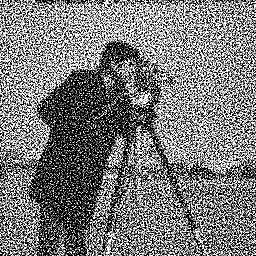
\includegraphics[width=0.30\textwidth]{question6/3_cam_wnr0_001}
	}
	\subfigure[NSR=0.01; PSNR +13.89dB]{
	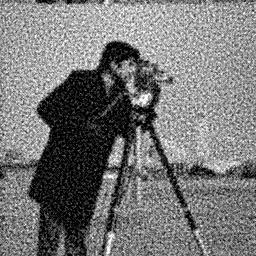
\includegraphics[width=0.30\textwidth]{question6/3_cam_wnr0_01}
	}
	\subfigure[NSR=0.05; PSNR +16.00dB]{
	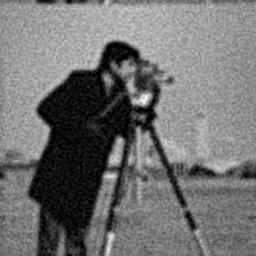
\includegraphics[width=0.30\textwidth]{question6/3_cam_wnr0_05}
	}
	
	\subfigure[NSR=0.1; PSNR +16.16dB]{
	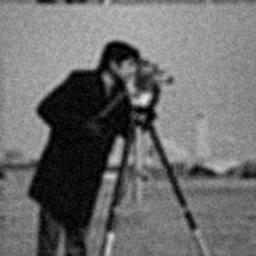
\includegraphics[width=0.30\textwidth]{question6/3_cam_wnr0_10}
	}
	\subfigure[NSR=0.2; PSNR +15.66dB]{
	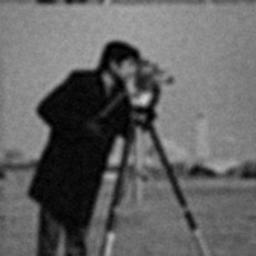
\includegraphics[width=0.30\textwidth]{question6/3_cam_wnr0_20}
	}
	\subfigure[NSR=0.4; PSNR +14.05dB]{
	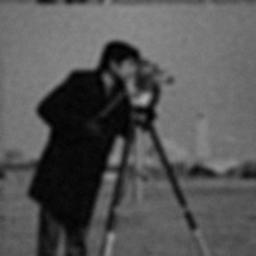
\includegraphics[width=0.30\textwidth]{question6/3_cam_wnr0_40}
	}
	\caption{Wiener filtering with various NSR. As NSR $\rightarrow$0, Wiener filtering becomes normal inverse filtering.}
\end{figure}


\subsubsection{Compare the restored image with the restored image from the previous step. How does the restored image and the PSNR differ from the previous restored image? Is it better or worse? Why? Explain it in context with the concept behind Wiener filtering.}

The restored image using the Wiener filter is much closer to the original (using NSR=0.1 as the best one) than the straight inverse filtering. Wiener filtering attenuates various frequencies when applying an inverse filter. As the noise in the image is relatively flat across all frequencies, the noise to signal ratio is approximated by a constant.

The Wiener filtering can be explained as blending the distorted image with noise with the inverse of the distorted image with noise. By reducing the inverse component, the issue of noise in deconvolution can be reduced.

\subsubsection{Can you draw any conclusions about Wiener filtering when applied to noise degraded images?}

Wiener filtering is able to accommodate noise when attempting to solve the noise problem inherent in deconvolution. The NSR, if unknown, must be carefully chosen in order to to get a good result.
